\mysection{The Knave}{trope-knave}

  \flavor{Fortune and glory, kid.  Fortune and glory. \Tilde Indiana Jones}

  \mysubsection{The Basics}{knave-basics}

  \myhighlight{Hale}{knave-flesh}

  Knaves start with d8 \FLESH 

  \myhighlight{Puissance}{knave-puissance}

  Knaves add their \LVL to any \RO or \RB attempt they're trying that includes their \DEX.  

  \myhighlight{Luck Dice}{knave-luck-die}

  Knaves have a Luck Die (d4 to start) - a unique \UD whose result can be applied to any \RO or \RB try that includes \DEX.  Roll the Luck Die and add its result to your \RO or \RB check.  You can only roll your Luck Die once per \RO or \RB

  \myhighlight{Whispers}{knave-whispers}

  Through sleight of hand, mind manipulation, minor illusion, complex gestures, and arcane words, Knaves are able to perform "superhuman" feats of thievery (climbing unclimbable walls, disguising themselves, passing through shadows, etc.)  These Arcana are collectively known as \mybold{Whispers}.  There are 4 Whispers in total (the Whispers of Anne Bonnny, the Whispers of Br'er Rabbit, the Whispers of Sun Wukong, and the Whispers of the Bride) - each a different Virtue - that a Knave can learn.

\cbreak

  \mysubsection{Creation}{knave-creation}

  \callout{
    \mynumlist {
      \item Move any of your core Skills \DCUP
      \item Move any of your core Saves \DCUP
      \item Give yourself a Luck Die of d4
      \item Pick \mybold{three} \mylink{Virtues}{knave-virtues} from the list below.  You can only pick each Virtue once.
      \item Pick \mybold{one} \mylink{Complication}{knave-complications} from the list below (or make up your own with the Arbiter!)
      \item Write down your Starting Gear
    }
  }



    \mytable{X}{
      \thead{\mysubsection{Virtues}{knave-virtues}} \\
    }{
      \mylink{Deadeye}{knave-virtue-deadeye} \\
      \mylink{Duelist}{knave-virtue-duelist} \\
      \mylink{Guilded}{knave-virtue-guilded} \\
      \mylink{Inked}{knave-virtue-inked} \\
      \mylink{Intangibles}{knave-virtue-intangibles} \\
      \mylink{Mummy's Curse}{knave-virtue-mummys-curse} \\
      \mylink{Whispers of Anne Bonny}{knave-virtue-anne-bonny}  \\
      \mylink{Whispers of Br'er Rabbit}{knave-virtue-brer-rabbit}  \\
      \mylink{Whispers of Sun Wukong}{knave-virtue-sun-wukong}  \\
      \mylink{Whispers of The Bride}{knave-virtue-the-bride}  \\
    }


    \myhighlight{Deadeye}{knave-virtue-deadeye}

    Requires you to know the \mylink{Whispers of The Bride}{knave-virtue-the-bride}.  If you're hidden and take an Action to Aim, you can \mylink{Murder}{knave-murder} with a Throw or Shoot weapon.

    \myhighlight{Duelist}{knave-virtue-duelist}

    You start the game with two Fast weapons of your choice (including the Knave's Sword).  You can use the Florentine Mighty Deed regardless of your \DEX

   \newpage

    \myhighlight{Guilded}{knave-virtue-guilded}

    You are the ex member of a Thieves' Guild. In addition to your starting gear, pick 3 items from the following list:
    \dashedbox {
      \mybullet {
        \item a suit of Light armor;
        \item a set of two silver daggers;
        \item a Bow and quiver of arrows (d10 \UD);
        \item 5 picks from the \mylink{Adventuring Gear}{gear-adventuring} table;
        \item a pouch of 3 gems (roll on the \mylink{Gems table}{appendixb-random-treasure} in Appendix B);
        \item d4 \UD of a Narcotic of your choice;
        \item a Fetish with d4 \UD of any spell you choose;
        \item d4 \UD of an Iron Toxin    
      }
    }

    Tell the Arbiter the name of your ex-Guild, and why you left ...    


    \myhighlight{Inked}{knave-virtue-inked}

    You start the game with all of the following \mylink{Tattoos}{research-inscription-tattoo}:  Dagger, Torch, Compass, and Rope


    \myhighlight{Intangibles}{knave-virtue-intangibles}

    You may move two different Intangible Stats of your choice \DCUP.  Describe to the Arbiter why these Intangible Stats are better than average.

    \myhighlight{Mummy's Curse}{knave-virtue-mummys-curse}

    You're immune to the effects of cursed or supernatural items you carry as long as you intend to sell them.  If you use the item or gain any benefit from it, you suffer the negative effects    

    \myhighlight{Whispers of Anne Bonny}{knave-virtue-anne-bonny}

    You know the whispers that help you climb walls, disguise yourself, forge documents, swing from chandeliers, and fight with two weapons.  See the section on \mylink{Arcana: Whispers}{arcana-whispers}

   \begin{center}
      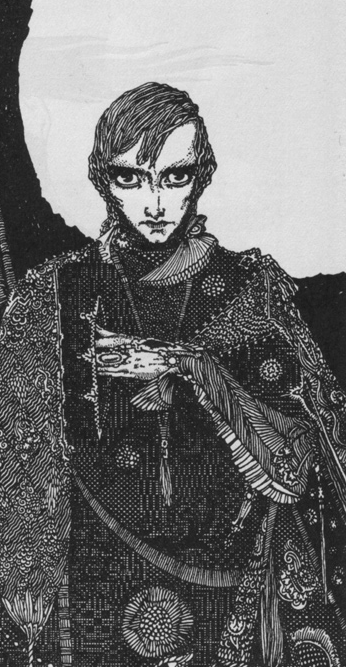
\includegraphics[scale=0.6]{Knave}
    \end{center}


    \myhighlight{Whispers of Br'er Rabbit}{knave-virtue-brer-rabbit}

    You know the whispers that help you pick pockets, escape prisons, perform sleight-of-hand, and cast spells from Fetishes.  See the section on \mylink{Arcana: Whispers}{arcana-whispers}

    \myhighlight{Whispers of Sun Wukong}{knave-virtue-sun-wukong}

    You know the whispers to hide things on your person, find and disarm traps, and open locks.   See the section on \mylink{Arcana: Whispers}{arcana-whispers}

    \myhighlight{Whispers of The Bride}{knave-virtue-the-bride}

    You know the whispers that help you move silently, hide in shadows, apply poisons, and murder your victims.   See the section on \mylink{Arcana: Whispers}{arcana-whispers}

 



    \mytable{X}{
      \thead{\mysubsection{Complications}{knave-complications}} \\
    }{
      Arch-nemesis \\
      Cursed \\
      Expensive Tastes \\
      Honor Among Thieves \\      
      Outstanding Contract \\
      Pacifist \\
      Pandemonium \\
      Religious \\
      Remorseless \\
      Superstitious \\
    }

    \myhighlight{Arch-Nemesis}{knave-complication-archnemesis}
    
    You have an arch-nemesis who always seems to be a step ahead of you when it comes to obtaining artifacts. Tell the Arbiter a little bit about them.

    \myhighlight{Cursed}{knave-complication-cursed}

    Probably should have left that amulet alone.  Roll on the {Lesser Curses}{table-lesser-curses} table - you start the game under that curse.  Tell the Arbiter how you acquired this curse.

    \myhighlight{Expensive Tastes}{knave-complication-tastes}

    You have exquisite and deviant tastes for the finer things in life. It costs you twice as much to take a \mylink{Vacation}{civilization-vacation}; the money spent is still applied to your experience.

    \myhighlight{Honor Among Thieves}{knave-complication-honor}

    You're a professional, and you appreciate other professionals.  You'll always give a hand to a fellow Knave even if that might inconvenience you or your \mylink{Band}{the-band}.

    \myhighlight{Outstanding Contract}{knave-complication-contract}

    There's an outstanding contract on your head, revenge for something you did.  Tell the Arbiter who is after you and why they want to kill you.

    \myhighlight{Pacifist}{knave-complication-pacifist}

    You won't ever start a fight (including stabbing someone unawares in the back).  You have no problems fighting once a fight is joined, however.  


    \myhighlight{Pandemonium}{knave-complication-pandemonium}

    You spend money as fast as you can make it, steal from the rich to give to the poor, and thrive in chaos.  You aren't motivated by anything material; you want anarchy, discord, and confusion.    

    \myhighlight{Religious}{knave-complication-religious}

    You are very religious (secretly or not).  You don't worship a specific Small God necessarily, but you have enormous respect for Mystics, \TheAuthority, and the Authorities.  You won't steal anything from a church or temple; priest of priestess - regardless of the Small God.


    \myhighlight{Remorseless}{knave-complication-remorseless}

    You feel nothing when you take a life or cause pain, but you suffer from \mylink{Night Terrors}{madness-night-terrors}.  This affliction can never be cured.


    \myhighlight{Superstitious}{knave-complication-superstitious}

    You are extremely superstitious (and believe this superstition has kept you alive up until now).  You fear the Jinx and prefer the company of Pooka whenever possible.  You won't steal from the dead, or take anything from tombs or graves.


    \mysubsection{Starting Gear}{knave-starting-gear}


    \mybullet {
      \item 10 iron pieces; 
      \item a set of belt pouches;
      \item d4 \UD of personal provisions;
      \item two daggers OR 1 short sword;
      \item one pick OR 3 rolls on the \mylink{Random Items}{appendixb-random-items} table in Appendix B;
    }

    \newpage

    \mysubsection{Examples}{knave-examples}

    \myhighlight{The Bandit}{knave-bandit}

    \example{Travel, Whispers of The Bride, Guild's Gift, Inked, Pandemonium}
    
    \myhighlight{The Assassin}{knave-assassin}

    \example{Listen, Whispers of The Bride, Whispers of Br'er Rabbit, Deadeye, Religious}
   
    \cbreak\bump

    \myhighlight{The Buccaneer}{knave-buccaneer}

    \example{Salt, Whispers of Anne Bonny, Duelist, Intangibles (Talent), Expensive Tastes}
   
    \myhighlight{The Archaeologist}{knave-archaeologist}

    \example{Lore, Mummy's Curse, Whispers of Br'er Rabbit, Whispers of Sun Wukong, Pacifist}

